% Paper B -- PRL DRAFT (revision of 2026-10-05: G2 is the discovery, G1 the
% setup, G3 the generality proof; paperB/plan.md is the submission map).
% Gates G1-G3 are preregistered, run and frozen (tags paperB-g2-freeze,
% paperB-g3-freeze); nothing scientific changes with the framing.
%
% Every number is a macro from numbers.tex, which docs/paperB/latex_tables.py
% regenerates from paperB/FROZEN.json. Nothing is typed by hand. `make check`
% enforces it and prints the core word count (APS: 3750 incl. figure
% equivalents; End Matter up to two pages, not counted).
%
% The submission will use revtex4-2; that class is not installed here, so the
% draft builds under article and the structure is what is being fixed.
\documentclass[11pt]{article}
\usepackage[margin=1in]{geometry}
\usepackage{graphicx}
\usepackage{amsmath}
\usepackage{natbib}
% generated by docs/paperB/latex_tables.py from paperB/FROZEN.json -- do not edit
\newcommand{\PBdmMax}{0.10}
\newcommand{\PBdcolMax}{0.10}
\newcommand{\PBGoneB}{GREEN}
\newcommand{\PBGoneDecision}{CONTINUE}
\newcommand{\PBGtwoHone}{GREEN}
\newcommand{\PBGtwoHtwo}{YELLOW}
\newcommand{\PBLaNgStar}{2}
\newcommand{\PBLaEpsStar}{0.20}
\newcommand{\PBLaEpsErr}{0.07}
\newcommand{\PBLaRerr}{0.036}
\newcommand{\PBLaEvPerPkt}{0.7}
\newcommand{\PBLaKlocal}{2}
\newcommand{\PBLaLstar}{0.504}
\newcommand{\PBLaShift}{0.07}
\newcommand{\PBLaRebuilt}{0.015}
\newcommand{\PBLaDownward}{0.06}
\newcommand{\PBLaSurvives}{yes}
\newcommand{\PBLaNExit}{524}
\newcommand{\PBLaNLines}{17{,}743}
\newcommand{\PBLaKbTables}{14}
\newcommand{\PBLaConc}{138}
\newcommand{\PBLaEventGlobal}{0.093}
\newcommand{\PBLaEventLocal}{0.311}
\newcommand{\PBLaBandGlobal}{0.034}
\newcommand{\PBLaBandLocal}{0.004}
\newcommand{\PBLaEventRatio}{3.4}
\newcommand{\PBLaBandRatio}{8.6}
\newcommand{\PBLaKglobal}{2}
\newcommand{\PBLaColourGlobal}{0.017}
\newcommand{\PBLaColourLocal}{0.006}
\newcommand{\PBLaEvO}{does not}
\newcommand{\PBLaEpsMM}{0.20}
\newcommand{\PBLaEpsMMErr}{0.07}
\newcommand{\PBLaEpsMMBand}{0.07}
\newcommand{\PBLaEpsMMColour}{0.07}
\newcommand{\PBLaEpsColour}{0.07}
\newcommand{\PBLaBuildS}{1}
\newcommand{\PBLaRefS}{1}
\newcommand{\PBLaOpS}{2}
\newcommand{\PBLaOpOverRef}{1.05}
\newcommand{\PBLaScalarOverRef}{4.2}
\newcommand{\PBLaOpKb}{16}
\newcommand{\PBLaMatrixB}{32}
\newcommand{\PBLaCostNg}{2}
\newcommand{\PBLaKernelEvents}{322{,}994}
\newcommand{\PBCeNgStar}{16}
\newcommand{\PBCeEpsStar}{0.00}
\newcommand{\PBCeEpsErr}{1.40}
\newcommand{\PBCeRerr}{0.060}
\newcommand{\PBCeEvPerPkt}{5.4}
\newcommand{\PBCeKlocal}{16}
\newcommand{\PBCeLstar}{0.358}
\newcommand{\PBCeShift}{2.09}
\newcommand{\PBCeRebuilt}{0.026}
\newcommand{\PBCeDownward}{1.96}
\newcommand{\PBCeSurvives}{yes}
\newcommand{\PBCeNExit}{12{,}510}
\newcommand{\PBCeNLines}{408{,}639}
\newcommand{\PBCeKbTables}{295}
\newcommand{\PBCeConc}{2{,}356}
\newcommand{\PBCeEventGlobal}{0.058}
\newcommand{\PBCeEventLocal}{0.138}
\newcommand{\PBCeBandGlobal}{0.081}
\newcommand{\PBCeBandLocal}{0.032}
\newcommand{\PBCeEventRatio}{2.4}
\newcommand{\PBCeBandRatio}{2.5}
\newcommand{\PBCeKglobal}{32}
\newcommand{\PBCeColourGlobal}{0.034}
\newcommand{\PBCeColourLocal}{0.051}
\newcommand{\PBCeEvO}{does}
\newcommand{\PBCeEpsMM}{0.00}
\newcommand{\PBCeEpsMMErr}{1.43}
\newcommand{\PBCeEpsMMBand}{1.40}
\newcommand{\PBCeEpsMMColour}{1.43}
\newcommand{\PBCeEpsColour}{1.43}
\newcommand{\PBCeBuildS}{12}
\newcommand{\PBCeRefS}{11}
\newcommand{\PBCeOpS}{13}
\newcommand{\PBCeOpOverRef}{1.15}
\newcommand{\PBCeScalarOverRef}{4.4}
\newcommand{\PBCeOpKb}{303}
\newcommand{\PBCeMatrixB}{2{,}048}
\newcommand{\PBCeCostNg}{16}
\newcommand{\PBCeKernelEvents}{5{,}439{,}289}
\newcommand{\PBNdNgStar}{2}
\newcommand{\PBNdEpsStar}{0.00}
\newcommand{\PBNdEpsErr}{1.06}
\newcommand{\PBNdRerr}{0.086}
\newcommand{\PBNdEvPerPkt}{8.2}
\newcommand{\PBNdKlocal}{2}
\newcommand{\PBNdLstar}{0.113}
\newcommand{\PBNdShift}{0.89}
\newcommand{\PBNdRebuilt}{0.046}
\newcommand{\PBNdDownward}{0.94}
\newcommand{\PBNdSurvives}{yes}
\newcommand{\PBNdNExit}{86{,}187}
\newcommand{\PBNdNLines}{3{,}336{,}077}
\newcommand{\PBNdKbTables}{2022}
\newcommand{\PBNdConc}{4{,}061}
\newcommand{\PBNdEventGlobal}{0.075}
\newcommand{\PBNdEventLocal}{0.132}
\newcommand{\PBNdBandGlobal}{0.162}
\newcommand{\PBNdBandLocal}{0.008}
\newcommand{\PBNdEventRatio}{1.8}
\newcommand{\PBNdBandRatio}{20.8}
\newcommand{\PBNdKglobal}{undefined}
\newcommand{\PBNdColourGlobal}{0.180}
\newcommand{\PBNdColourLocal}{0.010}
\newcommand{\PBNdEvO}{does not}
\newcommand{\PBNdEpsMM}{0.10}
\newcommand{\PBNdEpsMMErr}{0.82}
\newcommand{\PBNdEpsMMBand}{0.82}
\newcommand{\PBNdEpsMMColour}{0.75}
\newcommand{\PBNdEpsColour}{1.05}
\newcommand{\PBNdBuildS}{128}
\newcommand{\PBNdRefS}{127}
\newcommand{\PBNdOpS}{134}
\newcommand{\PBNdOpOverRef}{1.05}
\newcommand{\PBNdScalarOverRef}{4.1}
\newcommand{\PBNdOpKb}{2023}
\newcommand{\PBNdMatrixB}{32}
\newcommand{\PBNdCostNg}{2}
\newcommand{\PBNdKernelEvents}{18{,}641{,}032}
\newcommand{\PBContrastK}{32}
\newcommand{\PBParamsGlobal}{8{,}192}
\newcommand{\PBParamsLocal}{1{,}024}
\newcommand{\PBGthreeCone}{RED}
\newcommand{\PBGthreeCtwo}{RED}
\newcommand{\PBGthreeCthree}{YELLOW}
\newcommand{\PBGthreeCfour}{YELLOW}
\newcommand{\PBGthreeCfive}{GREEN}
\newcommand{\PBNgT}{16}
\newcommand{\PBNAxes}{4}
\newcommand{\PBNStatesPerIon}{14}
\newcommand{\PBLaCone}{GREEN}
\newcommand{\PBLaCtwo}{YELLOW}
\newcommand{\PBLaCthree}{GREEN}
\newcommand{\PBLaTransferHolds}{J}
\newcommand{\PBLaTransferFails}{T, D, P}
\newcommand{\PBLaInterpPasses}{T, D, J, P}
\newcommand{\PBLaNStates}{14}
\newcommand{\PBLaNGray}{0}
\newcommand{\PBLaNFreshFail}{0}
\newcommand{\PBLaNFreshFailBand}{0}
\newcommand{\PBLaWorstFreshBand}{0.040}
\newcommand{\PBLaWorstFreshColour}{0.043}
\newcommand{\PBLaWorstColourOver}{0.000}
\newcommand{\PBLaLeastColourOver}{0.000}
\newcommand{\PBLaKrecMax}{2}
\newcommand{\PBLaFixD}{0.097}
\newcommand{\PBLaFreshD}{0.012}
\newcommand{\PBLaIntWD}{0.030}
\newcommand{\PBLaIntMD}{0.032}
\newcommand{\PBLaLamD}{0.48}
\newcommand{\PBLaClsD}{B}
\newcommand{\PBLaFixJ}{0.010}
\newcommand{\PBLaFreshJ}{0.015}
\newcommand{\PBLaIntWJ}{0.003}
\newcommand{\PBLaIntMJ}{0.011}
\newcommand{\PBLaLamJ}{0.53}
\newcommand{\PBLaClsJ}{A}
\newcommand{\PBLaFixP}{0.191}
\newcommand{\PBLaFreshP}{0.040}
\newcommand{\PBLaIntWP}{0.054}
\newcommand{\PBLaIntMP}{0.014}
\newcommand{\PBLaLamP}{0.44}
\newcommand{\PBLaClsP}{B}
\newcommand{\PBLaFixT}{0.155}
\newcommand{\PBLaFreshT}{0.003}
\newcommand{\PBLaIntWT}{0.010}
\newcommand{\PBLaIntMT}{0.020}
\newcommand{\PBLaLamT}{0.59}
\newcommand{\PBLaClsT}{B}
\newcommand{\PBCeCone}{RED}
\newcommand{\PBCeCtwo}{YELLOW}
\newcommand{\PBCeCthree}{YELLOW}
\newcommand{\PBCeTransferHolds}{none}
\newcommand{\PBCeTransferFails}{T, D, J, P}
\newcommand{\PBCeInterpPasses}{T, D, J, P}
\newcommand{\PBCeNStates}{14}
\newcommand{\PBCeNGray}{0}
\newcommand{\PBCeNFreshFail}{7}
\newcommand{\PBCeNFreshFailBand}{1}
\newcommand{\PBCeWorstFreshBand}{0.119}
\newcommand{\PBCeWorstFreshColour}{0.162}
\newcommand{\PBCeWorstColourOver}{0.062}
\newcommand{\PBCeLeastColourOver}{0.007}
\newcommand{\PBCeKrecMax}{32}
\newcommand{\PBCeFixD}{0.223}
\newcommand{\PBCeFreshD}{0.056}
\newcommand{\PBCeIntWD}{0.047}
\newcommand{\PBCeIntMD}{0.130}
\newcommand{\PBCeLamD}{0.48}
\newcommand{\PBCeClsD}{B}
\newcommand{\PBCeFixJ}{0.042}
\newcommand{\PBCeFreshJ}{0.083}
\newcommand{\PBCeIntWJ}{0.050}
\newcommand{\PBCeIntMJ}{0.052}
\newcommand{\PBCeLamJ}{0.53}
\newcommand{\PBCeClsJ}{A}
\newcommand{\PBCeFixP}{0.231}
\newcommand{\PBCeFreshP}{0.068}
\newcommand{\PBCeIntWP}{0.084}
\newcommand{\PBCeIntMP}{0.093}
\newcommand{\PBCeLamP}{0.44}
\newcommand{\PBCeClsP}{B}
\newcommand{\PBCeFixT}{0.188}
\newcommand{\PBCeFreshT}{0.066}
\newcommand{\PBCeIntWT}{0.064}
\newcommand{\PBCeIntMT}{0.099}
\newcommand{\PBCeLamT}{0.59}
\newcommand{\PBCeClsT}{B}
\newcommand{\PBNdCone}{GREEN}
\newcommand{\PBNdCtwo}{RED}
\newcommand{\PBNdCthree}{GREEN}
\newcommand{\PBNdTransferHolds}{J}
\newcommand{\PBNdTransferFails}{T, D, P}
\newcommand{\PBNdInterpPasses}{T, D, J}
\newcommand{\PBNdNStates}{12}
\newcommand{\PBNdNGray}{2}
\newcommand{\PBNdNFreshFail}{0}
\newcommand{\PBNdNFreshFailBand}{0}
\newcommand{\PBNdWorstFreshBand}{0.033}
\newcommand{\PBNdWorstFreshColour}{0.050}
\newcommand{\PBNdWorstColourOver}{0.000}
\newcommand{\PBNdLeastColourOver}{0.000}
\newcommand{\PBNdKrecMax}{4}
\newcommand{\PBNdFixD}{0.375}
\newcommand{\PBNdFreshD}{0.013}
\newcommand{\PBNdIntWD}{0.034}
\newcommand{\PBNdIntMD}{0.110}
\newcommand{\PBNdLamD}{0.48}
\newcommand{\PBNdClsD}{B}
\newcommand{\PBNdFixJ}{0.035}
\newcommand{\PBNdFreshJ}{0.018}
\newcommand{\PBNdIntWJ}{0.026}
\newcommand{\PBNdIntMJ}{0.022}
\newcommand{\PBNdLamJ}{0.53}
\newcommand{\PBNdClsJ}{A}
\newcommand{\PBNdFixP}{0.181}
\newcommand{\PBNdFreshP}{0.013}
\newcommand{\PBNdIntWP}{0.117}
\newcommand{\PBNdIntMP}{0.057}
\newcommand{\PBNdLamP}{0.44}
\newcommand{\PBNdClsP}{C}
\newcommand{\PBNdFixT}{0.150}
\newcommand{\PBNdFreshT}{0.009}
\newcommand{\PBNdIntWT}{0.032}
\newcommand{\PBNdIntMT}{0.087}
\newcommand{\PBNdLamT}{0.59}
\newcommand{\PBNdClsT}{B}
\newcommand{\PBNdTrajAnchor}{0.181}
\newcommand{\PBNdTrajWhole}{0.117}
\newcommand{\PBNdTrajWholeColour}{0.075}
\newcommand{\PBNdTrajMatrix}{0.057}
\newcommand{\PBNdTrajMatrixColour}{0.110}
\newcommand{\PBNdTrajFresh}{0.013}
\newcommand{\PBNdTrajKrec}{2}
\newcommand{\PBNdTrajMatrixPasses}{fails}
\newcommand{\PBKmix}{undefined}
\newcommand{\PBKdirect}{4}
\newcommand{\PBAmixBestN}{16}
\newcommand{\PBAmixBestBand}{0.142}
\newcommand{\PBAmixBestColour}{0.131}
\newcommand{\PBAdirectBand}{0.083}
\newcommand{\PBAdirectColour}{0.053}
\newcommand{\PBBlendKrec}{4}
\newcommand{\PBBlendBand}{0.088}
\newcommand{\PBBlendColour}{0.073}
\newcommand{\PBBlendEps}{0.00}
\newcommand{\PBBlendEpsErr}{1.69}
\newcommand{\PBBlendNIons}{13}
\newcommand{\PBBlendEpsMM}{0.05}
\newcommand{\PBBlendEpsMMErr}{1.55}
\newcommand{\PBBlendEpsMMBand}{1.55}
\newcommand{\PBBlendEpsMMColour}{1.23}
\newcommand{\PBBlendEpsColour}{1.17}
\newcommand{\PBBlendBuildS}{193}
\newcommand{\PBBlendRefS}{187}
\newcommand{\PBBlendOpS}{176}
\newcommand{\PBBlendOpOverRef}{0.94}
\newcommand{\PBBlendScalarOverRef}{8.8}
\newcommand{\PBBlendOpKb}{4107}
\newcommand{\PBBlendMatrixB}{128}
\newcommand{\PBBlendExitLines}{175{,}086}
\newcommand{\PBBlendKernelEvents}{30{,}634{,}068}
\newcommand{\PBOpOverRefMin}{0.94}
\newcommand{\PBOpOverRefMax}{1.15}
\newcommand{\PBNdRtwoMOverRtwo}{1.8}
\newcommand{\PBGtwoR}{YELLOW}
\newcommand{\PBNScrambled}{31}
\newcommand{\PBNOrderings}{32}
\newcommand{\PBAdjCells}{10}
\newcommand{\PBAdjFirst}{8}
\newcommand{\PBAdjP}{0.031}
\newcommand{\PBCeGtwoR}{GREEN}
\newcommand{\PBCeAdjRank}{1}
\newcommand{\PBCeAdjFirstCells}{4}
\newcommand{\PBCeAdjNCells}{5}
\newcommand{\PBCeAdjE}{0.067}
\newcommand{\PBCeAdjScrMin}{0.140}
\newcommand{\PBCeAdjScrMedian}{0.204}
\newcommand{\PBCeAdjScrPass}{0\%}
\newcommand{\PBCeAdjNotFirst}{2}
\newcommand{\PBCeAdjETwo}{0.265}
\newcommand{\PBCeAdjMinTwo}{0.208}
\newcommand{\PBCeAdjMedTwo}{0.239}
\newcommand{\PBCeAdjRankTwo}{32}
\newcommand{\PBCeAdjEvRankTwo}{8}
\newcommand{\PBCeAdjEvTwo}{0.289}
\newcommand{\PBCeAdjEvMedTwo}{0.290}
\newcommand{\PBCeAdjEFour}{0.146}
\newcommand{\PBCeAdjMinFour}{0.186}
\newcommand{\PBCeAdjMedFour}{0.230}
\newcommand{\PBCeAdjRankFour}{1}
\newcommand{\PBCeAdjEvRankFour}{1}
\newcommand{\PBCeAdjEvFour}{0.244}
\newcommand{\PBCeAdjEvMedFour}{0.290}
\newcommand{\PBCeAdjEEight}{0.115}
\newcommand{\PBCeAdjMinEight}{0.183}
\newcommand{\PBCeAdjMedEight}{0.229}
\newcommand{\PBCeAdjRankEight}{1}
\newcommand{\PBCeAdjEvRankEight}{1}
\newcommand{\PBCeAdjEvEight}{0.238}
\newcommand{\PBCeAdjEvMedEight}{0.282}
\newcommand{\PBCeAdjESixteen}{0.067}
\newcommand{\PBCeAdjMinSixteen}{0.140}
\newcommand{\PBCeAdjMedSixteen}{0.204}
\newcommand{\PBCeAdjRankSixteen}{1}
\newcommand{\PBCeAdjEvRankSixteen}{1}
\newcommand{\PBCeAdjEvSixteen}{0.182}
\newcommand{\PBCeAdjEvMedSixteen}{0.256}
\newcommand{\PBCeAdjEThirtyTwo}{0.051}
\newcommand{\PBCeAdjMinThirtyTwo}{0.060}
\newcommand{\PBCeAdjMedThirtyTwo}{0.145}
\newcommand{\PBCeAdjRankThirtyTwo}{1}
\newcommand{\PBCeAdjEvRankThirtyTwo}{1}
\newcommand{\PBCeAdjEvThirtyTwo}{0.138}
\newcommand{\PBCeAdjEvMedThirtyTwo}{0.193}
\newcommand{\PBNdGtwoR}{YELLOW}
\newcommand{\PBNdAdjRank}{2}
\newcommand{\PBNdAdjFirstCells}{4}
\newcommand{\PBNdAdjNCells}{5}
\newcommand{\PBNdAdjE}{0.069}
\newcommand{\PBNdAdjScrMin}{0.068}
\newcommand{\PBNdAdjScrMedian}{0.091}
\newcommand{\PBNdAdjScrPass}{87\%}
\newcommand{\PBNdAdjNotFirst}{2}
\newcommand{\PBNdAdjETwo}{0.069}
\newcommand{\PBNdAdjMinTwo}{0.068}
\newcommand{\PBNdAdjMedTwo}{0.091}
\newcommand{\PBNdAdjRankTwo}{2}
\newcommand{\PBNdAdjEvRankTwo}{2}
\newcommand{\PBNdAdjEvTwo}{0.189}
\newcommand{\PBNdAdjEvMedTwo}{0.191}
\newcommand{\PBNdAdjEFour}{0.063}
\newcommand{\PBNdAdjMinFour}{0.073}
\newcommand{\PBNdAdjMedFour}{0.087}
\newcommand{\PBNdAdjRankFour}{1}
\newcommand{\PBNdAdjEvRankFour}{1}
\newcommand{\PBNdAdjEvFour}{0.172}
\newcommand{\PBNdAdjEvMedFour}{0.192}
\newcommand{\PBNdAdjEEight}{0.032}
\newcommand{\PBNdAdjMinEight}{0.054}
\newcommand{\PBNdAdjMedEight}{0.087}
\newcommand{\PBNdAdjRankEight}{1}
\newcommand{\PBNdAdjEvRankEight}{1}
\newcommand{\PBNdAdjEvEight}{0.169}
\newcommand{\PBNdAdjEvMedEight}{0.187}
\newcommand{\PBNdAdjESixteen}{0.016}
\newcommand{\PBNdAdjMinSixteen}{0.049}
\newcommand{\PBNdAdjMedSixteen}{0.081}
\newcommand{\PBNdAdjRankSixteen}{1}
\newcommand{\PBNdAdjEvRankSixteen}{2}
\newcommand{\PBNdAdjEvSixteen}{0.153}
\newcommand{\PBNdAdjEvMedSixteen}{0.166}
\newcommand{\PBNdAdjEThirtyTwo}{0.010}
\newcommand{\PBNdAdjMinThirtyTwo}{0.028}
\newcommand{\PBNdAdjMedThirtyTwo}{0.064}
\newcommand{\PBNdAdjRankThirtyTwo}{1}
\newcommand{\PBNdAdjEvRankThirtyTwo}{27}
\newcommand{\PBNdAdjEvThirtyTwo}{0.132}
\newcommand{\PBNdAdjEvMedThirtyTwo}{0.121}
\newcommand{\PBUCases}{33}
\newcommand{\PBURecords}{18}
\newcommand{\PBUSeeds}{12}
\newcommand{\PBUBoot}{10{,}000}
\newcommand{\PBUWinLo}{0.07}
\newcommand{\PBUWinHi}{0.13}
\newcommand{\PBUPass}{5}
\newcommand{\PBUFail}{13}
\newcommand{\PBUNoise}{13}
\newcommand{\PBUGray}{2}
\newcommand{\PBUFlips}{7}
\newcommand{\PBUNdTrajWhole}{0.118}
\newcommand{\PBUNdTrajWholeLo}{0.113}
\newcommand{\PBUNdTrajWholeHi}{0.123}
\newcommand{\PBUNdTrajWholeP}{0\%}
\newcommand{\PBUNdTrajWholeFrozen}{0.117}
\newcommand{\PBUNdTrajWholeStatus}{decided fail}
\newcommand{\PBUNdTrajMatrix}{0.119}
\newcommand{\PBUNdTrajMatrixLo}{0.110}
\newcommand{\PBUNdTrajMatrixHi}{0.130}
\newcommand{\PBUNdTrajMatrixP}{0\%}
\newcommand{\PBUNdTrajMatrixFrozen}{0.110}
\newcommand{\PBUNdTrajMatrixStatus}{decided fail}
\newcommand{\PBUCeJFix}{0.086}
\newcommand{\PBUCeJFixLo}{0.065}
\newcommand{\PBUCeJFixHi}{0.108}
\newcommand{\PBUCeJFixP}{88\%}
\newcommand{\PBUCeJFixFrozen}{0.107}
\newcommand{\PBUCeJFixStatus}{within noise}
\newcommand{\PBUCeTFresh}{0.122}
\newcommand{\PBUCeTFreshLo}{0.100}
\newcommand{\PBUCeTFreshHi}{0.146}
\newcommand{\PBUCeTFreshP}{2\%}
\newcommand{\PBUCeTFreshFrozen}{0.084}
\newcommand{\PBUCeTFreshStatus}{decided fail}
\newcommand{\PBUCePFresh}{0.137}
\newcommand{\PBUCePFreshLo}{0.127}
\newcommand{\PBUCePFreshHi}{0.149}
\newcommand{\PBUCePFreshP}{0\%}
\newcommand{\PBUCePFreshFrozen}{0.151}
\newcommand{\PBUCePFreshStatus}{gray}
\newcommand{\PBUBlend}{0.095}
\newcommand{\PBUBlendLo}{0.080}
\newcommand{\PBUBlendHi}{0.111}
\newcommand{\PBUBlendP}{70\%}
\newcommand{\PBUBlendFrozen}{0.088}
\newcommand{\PBUBlendStatus}{within noise}
\newcommand{\PBUAdirect}{0.071}
\newcommand{\PBUAdirectLo}{0.065}
\newcommand{\PBUAdirectHi}{0.084}
\newcommand{\PBUAdirectP}{100\%}
\newcommand{\PBUAdirectFrozen}{0.083}
\newcommand{\PBUAdirectStatus}{decided pass}


\title{Effective line redistribution in kilonova ejecta:\\
       transport-relevant structure is frequency-local}
\author{(author list to be fixed)}
\date{Draft, \today}

\begin{document}
\maketitle

\begin{abstract}
A reduced model of a many-body process is usually judged by how well it
reproduces the microscopic dynamics it replaces. We show, for lanthanide
line fluorescence in kilonova ejecta, that this criterion selects the wrong
model. Holding the atomic physics, the resolved line opacity and the
physical state fixed, we compare two reduced representations of the
redistribution of absorbed energy across frequency: a coarse graining into
contiguous frequency groups, and a global non-negative factorisation with
the same number of archetypal exit distributions and many more free
parameters. The global representation reproduces the microscopic
redistribution events \PBNdEventRatio\ times better and the emergent
broad-band light \PBNdBandRatio\ times worse. Frequency locality, not
fidelity to the microscopic distribution, is the structure the radiation
samples. The local operator reaches a \PBdmMax~mag photometric criterion
with a handful of groups where the best scalar thermalisation closure
misses by more than a magnitude; it remains compact across gas
temperature, density, illumination and a realistic \PBBlendNIons-ion
mixture, where \PBBlendKrec\ groups suffice and the scalar closure misses
by \PBBlendEpsErr~mag; but it is state dependent, interpolable along single
state coordinates and not along a coupled trajectory, and for one ion its
required resolution changes with the state.
\end{abstract}

\section{Introduction}
\label{sec:intro}
When a process with millions of microscopic degrees of freedom is replaced
by a reduced model, the reduction is normally built and judged against the
microscopic dynamics: the reduced model that reconstructs the fine-grained
process most accurately is taken to be the best. Goal-oriented model
reduction has long recognised that the appropriate reduced model can
depend on the quantity one wants from it \citep{benner2015}, and reduced
and low-rank formulations of radiative transfer exist \citep{peng2020}. The
question we address is narrower and physical: in a concrete transport
problem where the microscopic process can be simulated exactly, which of
its degrees of freedom actually reach the observable radiation, and does
fidelity to the microscopic process identify them?

The process is lanthanide line fluorescence in the ejecta of a neutron-star
merger. The open $f$-shells of the lanthanides carry of order $10^6$
transitions per ion at the relevant temperatures \citep{barneskasen2013,
tanaka2020}; a photon absorbed in one line is re-emitted, after a cascade
through the ion's levels, in another, and this redistribution of energy
across frequency is the dominant non-local process shaping a kilonova's
light. High-fidelity transport keeps the identity of every transition for
exactly this reason: line-by-line calculations with tens of millions of
lines follow the absorption and the cascade explicitly, through a
stochastic macroatom \citep{lucy2002,lucy2003,shingles2023}. Cheaper
calculations replace the cascade by a parameterised redistribution --- a
scalar thermalisation probability $\epsilon$ that sends a fraction of the
absorbed energy to a thermal pool and scatters the rest coherently, or a
frequency-grouped treatment of the opacity with a prescribed re-emission
within each group \citep{fontes2020}. Frequency redistribution as a
formalism is classical \citep{hummer1962}; what is not known is how much
of the fluorescence response a transport calculation needs, and what
organises the part it needs.

We hold the opacity at the resolved Sobolev value of every line, take an
energy-conserving downward macroatom as the exact reference, and build
reduced operators from the reference's own events on one set of random
seeds, scoring them on another. Three preregistered gates then ask, in
order, whether a compact operator exists where the scalar closure fails
(Section~\ref{sec:compression}); whether the structure it exploits is
locality in frequency or a globally low rank of the redistribution law
(Section~\ref{sec:mechanism}); and whether that structure survives changes
of state and composition (Section~\ref{sec:generality}). The second gate is
the result of this Letter. At matched complexity, the representation that
reproduces the microscopic redistribution better reproduces the light
worse, and the data identify frequency locality as the missing organising
principle. In lanthanide fluorescence transport, generic fidelity to the
microscopic redistribution does not identify the degrees of freedom that
control the emergent radiation; a frequency-local representation does.

\section{Set-up}
\label{sec:method}
Every calculation is a single-zone transport through the photospheric
shell of a published lanthanide-rich ejecta model at two days, with the
shell's own density, gas temperature and expansion time and a black-body
core illuminating it. One ion at a time --- La\,\textsc{ii},
Ce\,\textsc{ii} or Nd\,\textsc{ii}, at its number density in the shell, with
levels and lines from a calibrated atomic data set \citep{gsi_atomic} and
populations in local thermodynamic equilibrium --- carries the opacity;
La\,\textsc{ii} is thin enough at its partial density that every closure
agrees, and is a control. Packets carry indivisible energy. The reference
is a downward macroatom: on absorption the packet walks the radiative
cascade with branching probabilities $A\beta$ until it exits in a line
whose photon escapes, conserving energy at every step; the identity
between injected and accounted energy is verified to $10^{-10}$ on every
run.

The reduced operator is built from the reference's events (absorbed
frequency, exit frequency, energy before and after). On $N_g$ log-spaced
frequency groups, $R_{ij}$ is the fraction of energy absorbed in group $i$
that exits in group $j$; within each output group the exit line is drawn
from a discrete table of the distinct exit lines the events populated,
weighted by energy. Transport with the operator replaces the cascade by one
draw from $R_{ij}$ and one from the table. Operators are built on three
seeds and scored on three disjoint seeds. The global family of
Section~\ref{sec:mechanism} replaces the transition matrix by a rank-$k$
non-negative factorisation of the fine-grouped matrix on the same exit
tables; the state-dependent operators of Section~\ref{sec:generality} are
rebuilt at, transported to, or interpolated between states as described
there. Every closure is scored by its maximum absolute error in the
broad-band magnitudes and colours over the bands that carry at least one
per cent of the luminosity, by an integrated spectral distance, and by an
energy-weighted total-variation distance to an independent fine-grouped
matrix from the evaluation events; the criterion throughout is
\PBdmMax~mag in band and \PBdcolMax~mag in colour. The gates, their
readings and the amendments made during the runs are in the End Matter.

\section{A compact operator exists where a scalar closure fails}
\label{sec:compression}
The optimally tuned scalar misses the reference by \PBCeEpsErr~mag on
Ce\,\textsc{ii} and \PBNdEpsErr~mag on Nd\,\textsc{ii}; the group operator
meets the criterion at $N_g=\PBCeNgStar$ and $N_g=\PBNdNgStar$
(Fig.~\ref{fig:compression}a). The compression is not an artefact of one
cascade prescription: replacing the reference by a radiation-field-driven
macroatom with internal upward transitions moves the photometry by
\PBCeShift~mag on Ce\,\textsc{ii}, and an operator rebuilt from that
reference follows it to \PBCeRebuilt~mag while the operator trained on the
original reference stays \PBCeDownward~mag away
(Fig.~\ref{fig:compression}b). The operator carries the fluorescence
physics it is built from. This establishes that there is a non-trivial
reduced model to explain; the explanation is the next section.

\begin{figure}[t]
\centering
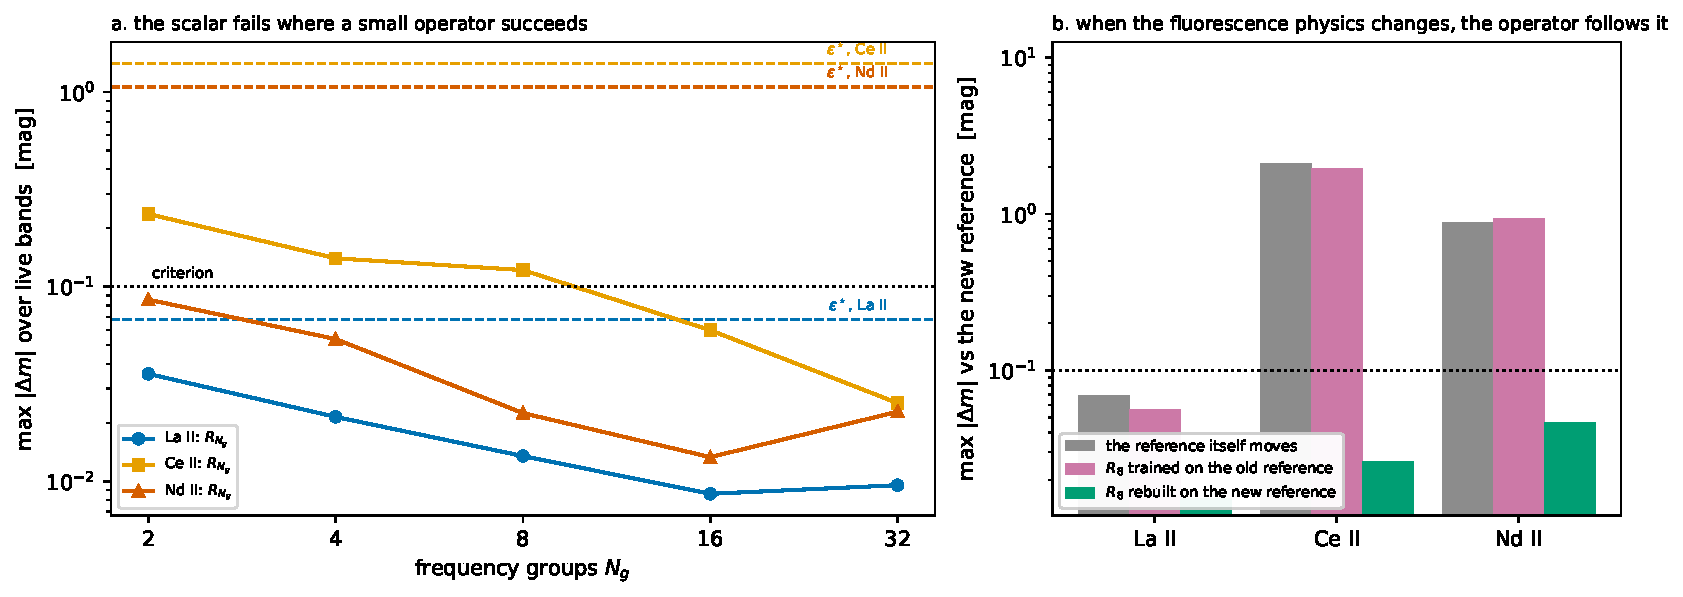
\includegraphics[width=\textwidth]{figures/fig1_compression.pdf}
\caption{\textbf{A scalar closure fails where a small operator succeeds,
and the operator follows the fluorescence physics.} (a) Maximum
photometric error against the energy-conserving downward macroatom for the
group operator at $N_g=2\ldots32$ (solid) and the optimally tuned scalar
$\epsilon^\star$ (dashed). (b) Under a radiation-field-driven macroatom the
reference itself moves (grey); an operator rebuilt from its events follows
it (green); the operator trained on the previous reference does not
(pink).}
\label{fig:compression}
\end{figure}

\section{Observable fidelity is not microscopic fidelity}
\label{sec:mechanism}
Two families of operator were built on identical exit tables and identical
opacity, differing only in the group-to-group matrix: local coarsening into
$N_g$ contiguous frequency blocks, and a global non-negative factorisation
into $k$ archetypal exit distributions mixed freely for every fine input
group. The matched axis is the number of archetypes. At equal count the
global family is far the more expressive, with \PBParamsGlobal\ free
numbers against \PBParamsLocal\ at \PBContrastK\ archetypes, and it fits
the microscopic redistribution better by construction. If the compression
of Section~\ref{sec:compression} reflected a globally low-rank
redistribution law, the global family would reach the photometric
criterion with fewer archetypes.

It does not. On Ce\,\textsc{ii} the local operator passes at
\PBCeKlocal\ archetypes and the global one at \PBCeKglobal; on
Nd\,\textsc{ii} the local operator passes at \PBNdKlocal\ and the global
family is \PBNdKglobal\ at every rank tried. The contrast is sharpest where
both are measured at the same count. At \PBContrastK\ archetypes on
Nd\,\textsc{ii} the global operator's event-level total-variation loss is
\PBNdEventGlobal\ against the local operator's \PBNdEventLocal, and its
photometric error is \PBNdBandGlobal~mag against \PBNdBandLocal~mag:
\begin{equation}
E_{\rm micro}^{\rm global} < E_{\rm micro}^{\rm local},\qquad
E_{\rm obs}^{\rm global} > E_{\rm obs}^{\rm local},
\label{eq:inversion}
\end{equation}
by factors of \PBNdEventRatio\ and \PBNdBandRatio\ respectively, and the
same inversion holds on every ion (Fig.~\ref{fig:mechanism}). The degrees
of freedom that minimise a generic distance between microscopic
redistribution distributions are not the degrees of freedom that carry the
radiation field. What the radiation samples is that neighbouring absorbed
frequencies share a transport-relevant response: an operator that keeps
contiguous frequencies together reproduces the light with a few blocks,
and a factorisation free to mix distant frequencies, however well it
reconstructs the events, does not.

The compression is two-level. Writing
$P(\nu_{\rm out}\mid\nu_{\rm in}) = P(j\mid i)\,P(\nu_{\rm out}\mid i,j)$,
the first factor is extremely coarse, while the second still needs a sparse
but real set of exit lines: truncating the exit tables by retained energy,
the light needs \PBCeLstar\ of the distinct exit lines on Ce\,\textsc{ii}
and \PBNdLstar\ on Nd\,\textsc{ii} at the same thresholds. We do not claim
that the atomic network has only a handful of degrees of freedom. We claim
that the part of it the transport needs is organised by frequency locality,
and that microscopic reconstruction error does not find it.

\begin{figure}[t]
\centering
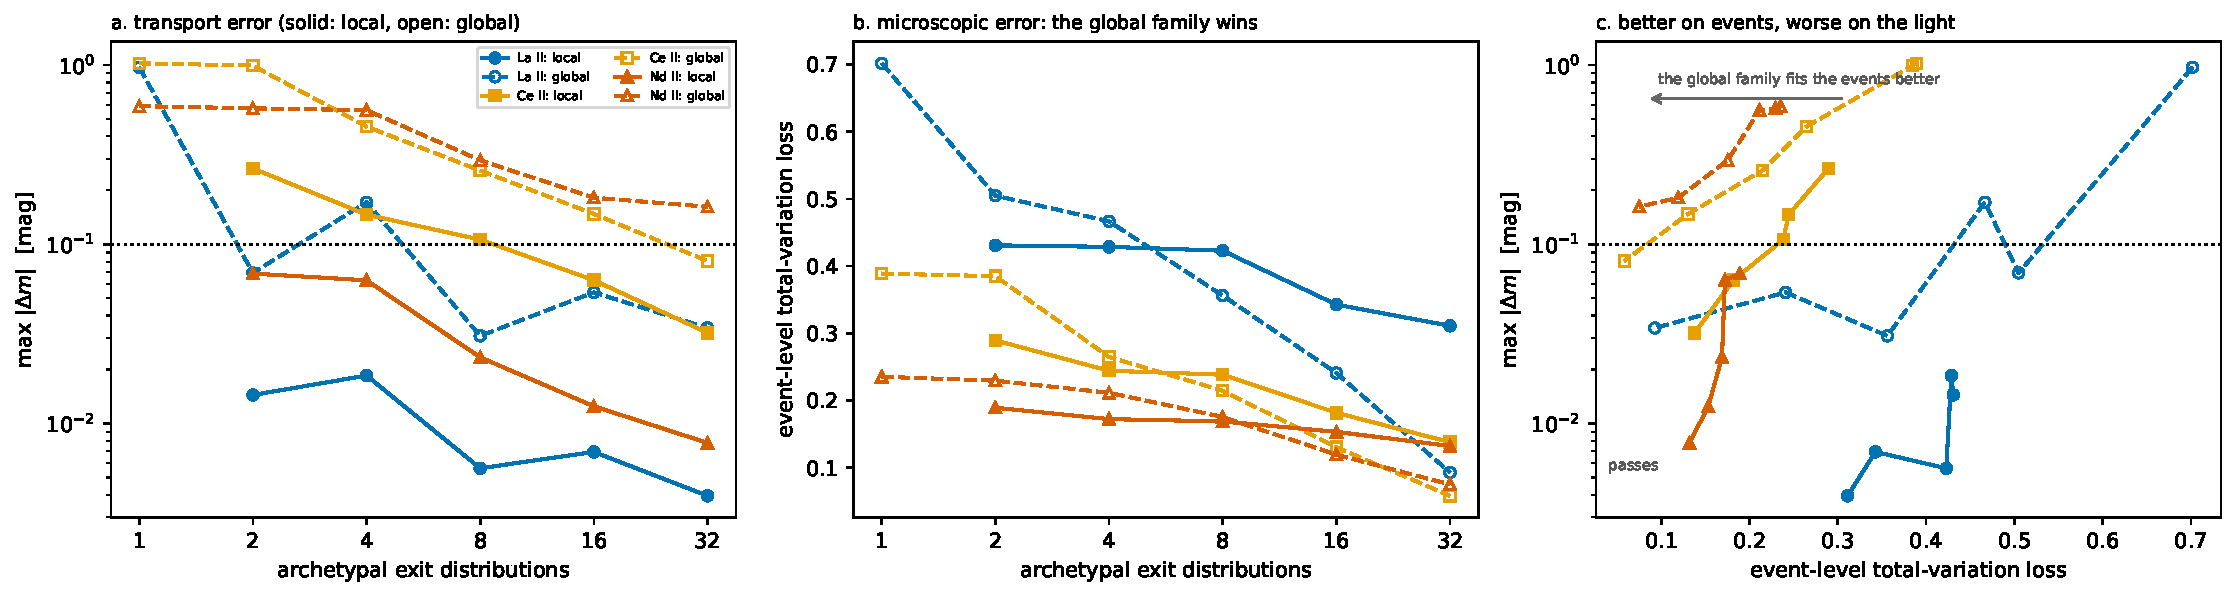
\includegraphics[width=\textwidth]{figures/fig2_mechanism.pdf}
\caption{\textbf{Better on the microscopic events, worse on the light.}
(a) Photometric error and (b) event-level total-variation loss against the
number of archetypal exit distributions, for local frequency coarsening
(solid) and the global factorisation (open). (c) The two against each
other: the global points move left, fitting the microscopic redistribution
better, while staying high, reproducing the emergent light worse.}
\label{fig:mechanism}
\end{figure}

\section{A state-dependent family, compact throughout}
\label{sec:generality}
Is the local operator a property of the ion or of the state it was built
in? We moved one coordinate at a time from the original state along
\PBNAxes\ axes --- gas temperature, number density, the temperature of the
illuminating source, and the physical trajectory at one, three and five
days along which all of them move together --- and at each of
\PBNStatesPerIon\ states per ion scored, against that state's own
reference, both the original operator transported unchanged and an
operator rebuilt there (Fig.~\ref{fig:generality}), both at \PBNgT\ groups.
The transported operator is not predictive: it fails on every axis for
Ce\,\textsc{ii} and on all but the source-spectrum axis for the other two
ions. The rebuilt operator passes at every readable state of
Nd\,\textsc{ii} and La\,\textsc{ii}, with at most \PBNdKrecMax\ groups
needed anywhere on Nd\,\textsc{ii}. There is no universal $R_{ij}$; the
failure of transfer is not a failure of compression.

What varies is the content of a small operator, and it varies smoothly
along single coordinates. At the interior point of each axis an operator
interpolated linearly in the logarithm of the moved coordinate between the
two bracketing states --- transition rows, deposition channel and exit
tables on the union of the endpoints' exit lines, never using the interior
state's events --- passes the criterion on the temperature, density and
source axes for every ion, reducing Nd\,\textsc{ii}'s error at the interior
temperature from \PBNdFixT\ to \PBNdIntWT~mag. The useful object is a
tabulated family $R(\theta)$. Its boundary is the coupled trajectory: at
three days on Nd\,\textsc{ii} the transported operator misses by
\PBNdTrajAnchor~mag, the interpolant by \PBNdTrajWhole~mag, and only the
operator rebuilt there passes, at \PBNdTrajKrec\ groups with
\PBNdTrajFresh~mag. The family is compact but not separable in
independently varied coordinates; interpolation was tested one axis at a
time and the one coupled path tested breaks it. Ce\,\textsc{ii} adds a
second qualification: its rebuilt \PBNgT-group operator fails at
\PBCeNFreshFail\ of \PBCeNStates\ states, on colour, by at most
\PBCeWorstColourOver~mag, and a \PBCeKrecMax-group operator passes at
every one. Compactness survives; a fixed representation size does not.

Composition closes the argument. Three single-ion operators combined by an
opacity-share rule, with no fit to the blend, do not reach the criterion at
any valid resolution (\PBAmixBestBand~mag at best), while an operator
built on the three-ion blend passes at \PBKdirect\ groups: per-species
operators do not compose. Yet on the full \PBBlendNIons-ion composition of
the benchmark state --- the mixture a transport calculation actually needs
--- the operator built on the blend passes at \PBBlendKrec\ groups
(\PBBlendBand~mag in band, \PBBlendColour\ in colour) while the best scalar
closure misses by \PBBlendEpsErr~mag, the widest scalar failure in this
work. The combined physical system is itself highly compressible even
though it cannot be assembled from its parts.

\begin{figure}[t]
\centering
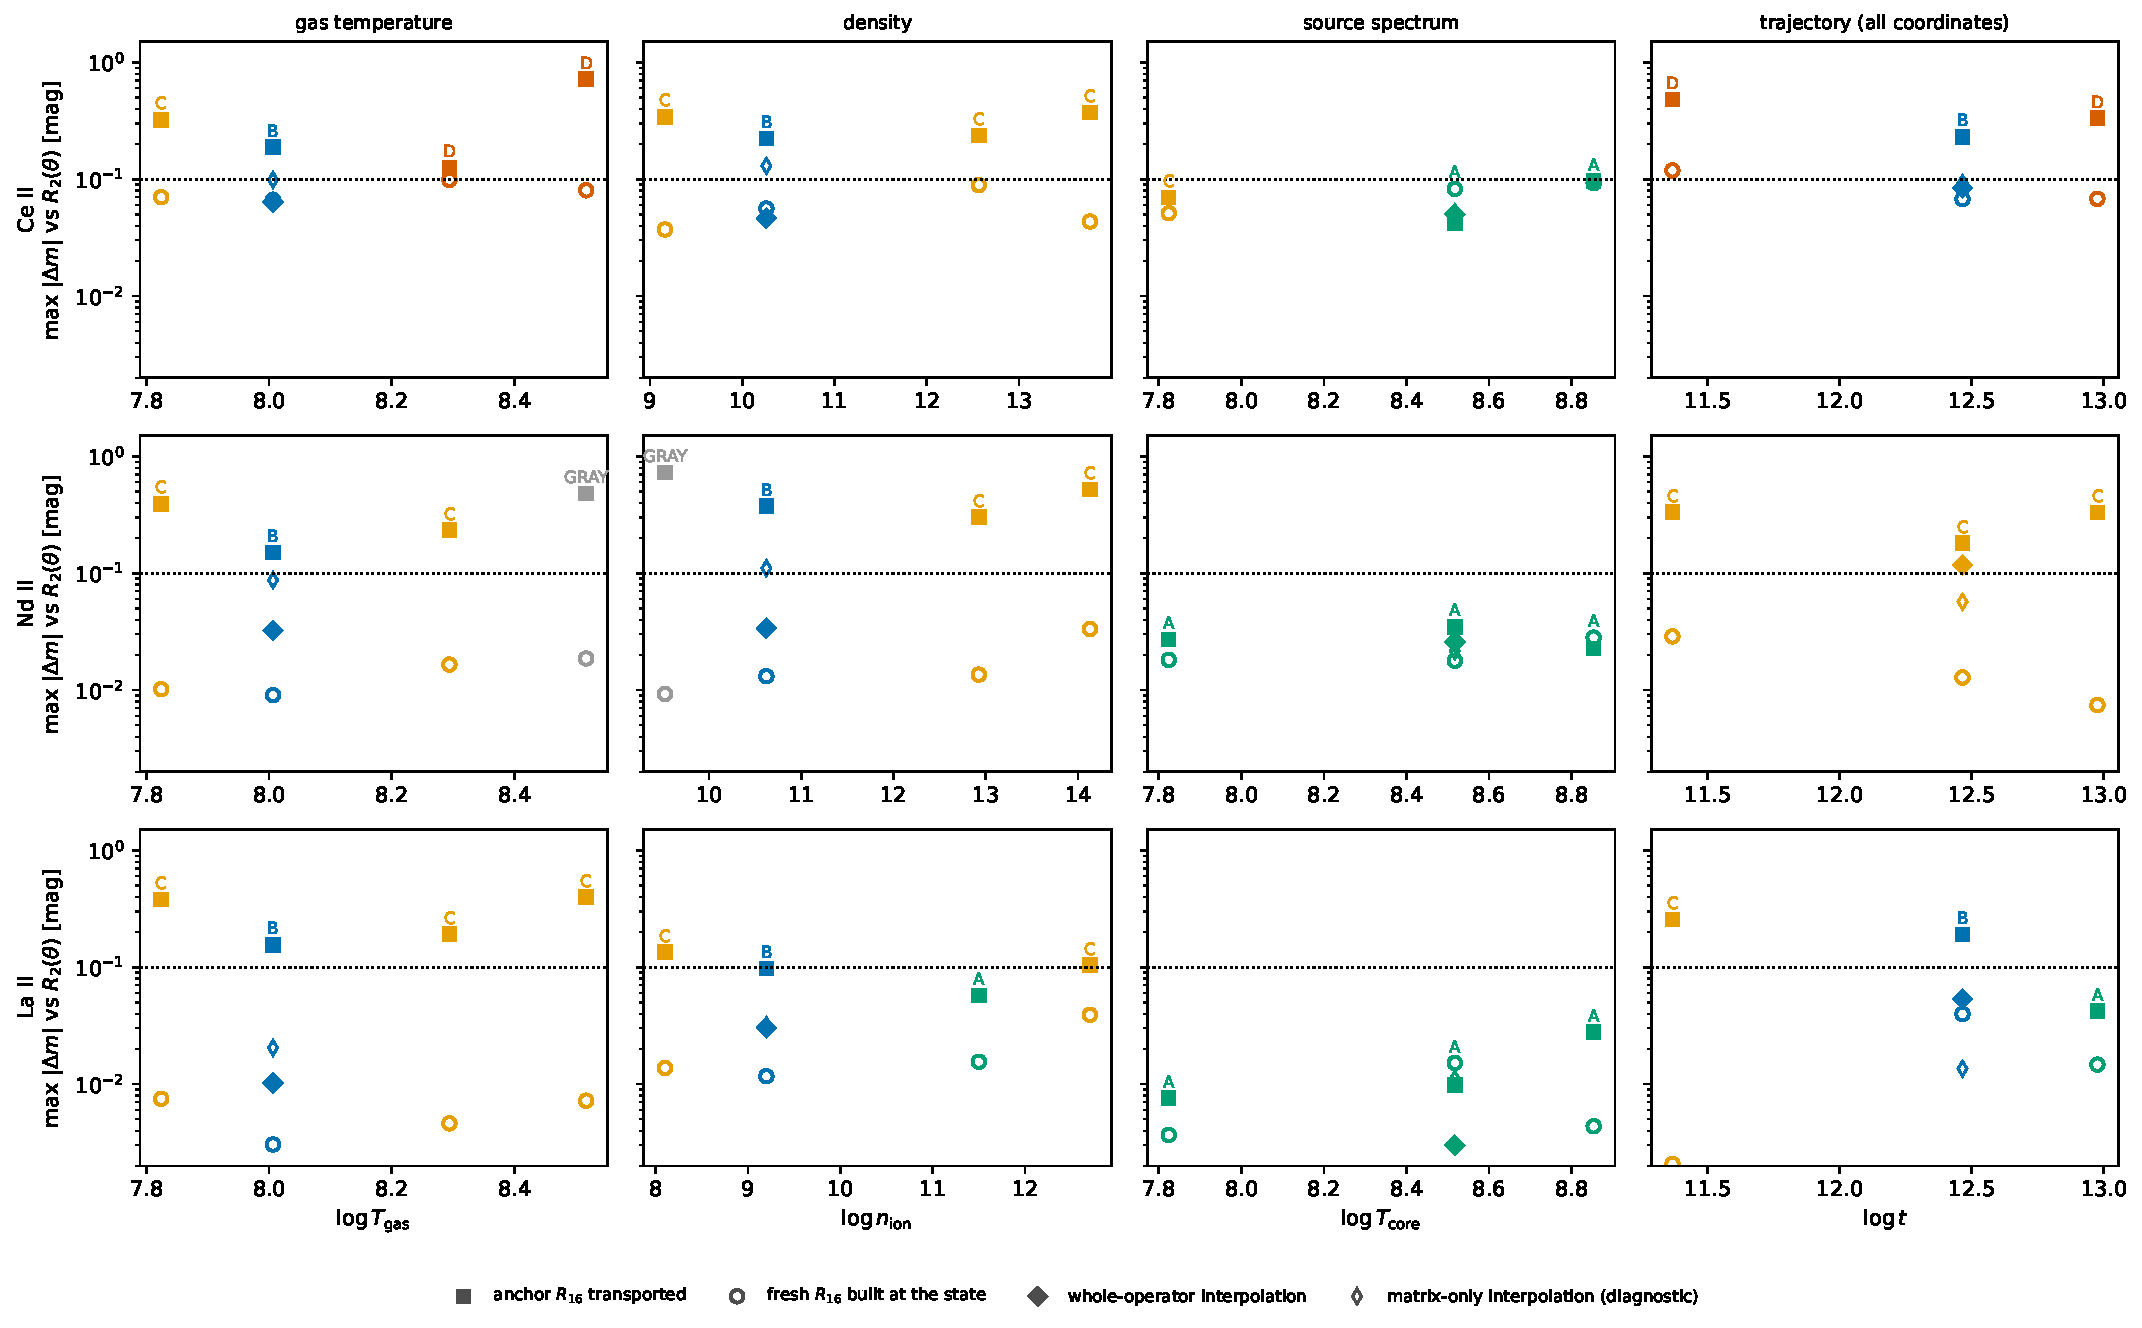
\includegraphics[width=\textwidth]{figures/fig3_generality.pdf}
\caption{\textbf{Transfer is not compression.} Maximum photometric error
against the state's own reference for the original operator transported
unchanged (filled squares), the operator rebuilt at the state (open
circles), and at each axis' interior point the whole-operator interpolant
from the two bracketing states (filled diamonds; matrix-only interpolant,
open diamonds). Rows: Ce\,\textsc{ii}, Nd\,\textsc{ii}, the La\,\textsc{ii}
control; columns: gas temperature, density, source spectrum, and the
trajectory along which all move together. Dotted: the band criterion; the
letter is the preregistered reading of each state (A transported operator
passes; B only the interpolant; C only a fresh fit; D none at \PBNgT\
groups). The criterion also bounds the colour error, so a circle below the
line can read D. Grey: states excluded by the preregistered validity
checks.}
\label{fig:generality}
\end{figure}

\section{Conclusions}
\label{sec:discussion}
Of the order $10^6$ transitions of a lanthanide ion, the transport sees a
fine distribution of redistribution events; of that distribution, the
emergent light sees a small frequency-local operator; and most of the
information between the two is discarded without harm. The decisive
evidence is the inversion of Eq.~(\ref{eq:inversion}): a representation
that reproduces the microscopic redistribution better reproduces the light
worse, so the microscopic distribution is the wrong target for a reduced
model of this process and frequency locality is the right one. The local
operator is not universal --- it is a state-dependent family, interpolable
along single coordinates, refit where coordinates move together, with a
resolution that is itself state-dependent for Ce\,\textsc{ii} --- and it
does not compose from single species; but on the realistic mixture it is
as compact as on any single ion. The limitations are those of the
set-up: single-zone, time-independent, with the radiation field imposed
and its influence measured only through the source-spectrum axis, on one
coupled path. None of them touches the inversion, which is measured on
identical events, identical opacity and identical observables. Transport
can discard most of the microscopic fluorescence information --- but only
if the reduced coordinates respect the structure the radiation actually
samples.

\section*{End Matter}
\label{sec:endmatter}

\paragraph{The gates.} Each of the three questions was preregistered as a
gate --- the state, the grids, the metrics, the thresholds, the gray
conditions that invalidate a reading and the readings themselves fixed and
committed before the run --- and read gray-first.
Table~\ref{tab:gates} gives the per-ion readings of the first gate (the
group count at which the operator meets the criterion, the best scalar and
its error) and of the second (the archetype counts of the local and global
families, and the fraction of exit lines the light needs), with the
robustness check against the radiation-field-driven macroatom;
Table~\ref{tab:contrast} the microscopic and observable errors of
Eq.~(\ref{eq:inversion}) at \PBContrastK\ archetypes on every ion;
Table~\ref{tab:generality} the third gate per ion --- its three readings,
the axes along which the transported operator stays predictive, how often
the rebuilt operator fails and the largest resolution it needed, and the
interpolation error at each single-coordinate interior point, whole
operator against transition matrix alone. The third gate's first reading
is Red for Ce\,\textsc{ii} (the resolution result above) and its second Red
for Nd\,\textsc{ii} (the trajectory); its mixture readings are Yellow for
composability and Green for the realistic blend.

\paragraph{Amendments during the runs.} Three were made and are recorded
in the archived preregistration with what had been seen when each was
made. In the second gate, two implementation defects in computing the
factorisation (a live row sent to zero; a fixed iteration count that had
not converged) were found on the control ion and fixed before any decisive
ion's numbers were read, and a validity control that compared the local
family on coarse and fine exit tables fired on both decisive ions and was
answered by its preregistered remedy, transporting the local family on the
shared fine tables; no threshold changed. In the third gate, an unclamped
cumulative-sum sampler overflowed on the \PBBlendNIons-ion mixture, the
largest line list in this work; it was fixed with the clip its sibling
samplers already carried, its reachability in every earlier record was
established by inspection (any overflow crashes, so no completed record
could have been affected), and the mixture calculation was repeated. A
separate, non-reproducible corruption of one energy-accounting sum in
three runs was audited by rerunning each, found not to affect the
photometry, and answered by excluding any run with an invalid energy
ledger from every reading.

\paragraph{Transport and validation.} The transport is a Monte Carlo
Sobolev code with worldline relativity and energy packets, developed and
validated in a companion methods paper on coarse line-opacity treatments
(in preparation). The properties this Letter relies on are verified
within it: the energy identity closes to $10^{-10}$ on every run reported;
the resolved Sobolev transport is pinned against a deterministic
formal-solution reference; the downward macroatom reproduces an explicit
cascade's energy per line; and every operator is built on seeds disjoint
from those it is scored on. The generality test lays every kernel of an ion
on one frequency support frozen over the whole state domain, so that an
operator transported between states is never clipped to a different range.

\paragraph{Data availability.} The transport code, the preregistrations of
the three gates, every run record, the frozen record from which every
number in this Letter is generated, and the scripts that regenerate the
numbers, tables and figures are archived at
\texttt{github.com/zhuygln/revisit\_sobolev} (tags \texttt{paperB-g2-prereg},
\texttt{paperB-g2-freeze}, \texttt{paperB-g3-prereg},
\texttt{paperB-g3-freeze}).

\begin{table}[p]
\centering
\caption{The first two gates, per ion.}
\label{tab:gates}
% generated by docs/paperB/latex_tables.py -- do not edit
\begin{tabular}{lccccccccc}
\hline
ion & $N_g^\star$ & $\epsilon^\star$ & error at $\epsilon^\star$ & $\epsilon^\star_{\rm mm}$ & $E_{\rm joint}(\epsilon^\star_{\rm mm})$ & $K^\star_{\rm local}$ & $K^\star_{\rm global}$ & $L^\star$ & $R_8$ vs the new reference \\
 & & & [mag] & & [mag] & & & & [mag] \\
\hline
La II & \PBLaNgStar & \PBLaEpsStar & \PBLaEpsErr & \PBLaEpsMM & \PBLaEpsMMErr & \PBLaKlocal & \PBLaKglobal & \PBLaLstar & \PBLaRebuilt \\
Ce II & \PBCeNgStar & \PBCeEpsStar & \PBCeEpsErr & \PBCeEpsMM & \PBCeEpsMMErr & \PBCeKlocal & \PBCeKglobal & \PBCeLstar & \PBCeRebuilt \\
Nd II & \PBNdNgStar & \PBNdEpsStar & \PBNdEpsErr & \PBNdEpsMM & \PBNdEpsMMErr & \PBNdKlocal & \PBNdKglobal & \PBNdLstar & \PBNdRebuilt \\
\hline
\end{tabular}

\end{table}

\begin{table}[p]
\centering
\caption{Microscopic against observable error at \PBContrastK\ archetypes.}
\label{tab:contrast}
% generated by docs/paperB/latex_tables.py -- do not edit
\begin{tabular}{lcccccc}
\hline
ion & $m_{\rm event}$ global & $m_{\rm event}$ local & max $|\Delta m|$ global & max $|\Delta m|$ local & max $|\Delta c|$ global & max $|\Delta c|$ local \\
 & & & [mag] & [mag] & [mag] & [mag] \\
\hline
La II & \PBLaEventGlobal & \PBLaEventLocal & \PBLaBandGlobal & \PBLaBandLocal & \PBLaColourGlobal & \PBLaColourLocal \\
Ce II & \PBCeEventGlobal & \PBCeEventLocal & \PBCeBandGlobal & \PBCeBandLocal & \PBCeColourGlobal & \PBCeColourLocal \\
Nd II & \PBNdEventGlobal & \PBNdEventLocal & \PBNdBandGlobal & \PBNdBandLocal & \PBNdColourGlobal & \PBNdColourLocal \\
\hline
\end{tabular}

\end{table}

\begin{table}[p]
\centering
\caption{The third gate, per ion: the readings, the axes along which the
transported operator stays predictive, how often the rebuilt \PBNgT-group
operator fails and the largest resolution it needed, and the
interior-point interpolation error (whole operator / transition matrix
only) on the three single-coordinate axes, in mag.}
\label{tab:generality}
% generated by docs/paperB/latex_tables.py -- do not edit
\begin{tabular}{lccccccccc}
\hline
ion & C1 & C2 & C3 & transfer holds & fresh $R_{16}$ fails & $\max K^\star_{\rm rec}$ & interp.\ $T$ & interp.\ $D$ & interp.\ $J$ \\
 & & & & (axes) & (of states) & & whole / matrix & whole / matrix & whole / matrix \\
\hline
La II & \PBLaCone & \PBLaCtwo & \PBLaCthree & \PBLaTransferHolds & \PBLaNFreshFail / \PBLaNStates & \PBLaKrecMax & \PBLaIntWT / \PBLaIntMT & \PBLaIntWD / \PBLaIntMD & \PBLaIntWJ / \PBLaIntMJ \\
Ce II & \PBCeCone & \PBCeCtwo & \PBCeCthree & \PBCeTransferHolds & \PBCeNFreshFail / \PBCeNStates & \PBCeKrecMax & \PBCeIntWT / \PBCeIntMT & \PBCeIntWD / \PBCeIntMD & \PBCeIntWJ / \PBCeIntMJ \\
Nd II & \PBNdCone & \PBNdCtwo & \PBNdCthree & \PBNdTransferHolds & \PBNdNFreshFail / \PBNdNStates & \PBNdKrecMax & \PBNdIntWT / \PBNdIntMT & \PBNdIntWD / \PBNdIntMD & \PBNdIntWJ / \PBNdIntMJ \\
\hline
\end{tabular}

\end{table}

\bibliographystyle{plainnat}
\bibliography{references}
\end{document}
